%************************************************
\chapter{Esempi e applicazioni}\label{cap:esempi}
%************************************************

In questo capitolo mostreremo alcuni esempi con dati sintetici che mostrano il tipo di visualizzazione che si riesce ad ottenere utilizzando l'omologia persistente, poi vedremo come la TDA è stata usata in diversi studi per ricostruire la struttura da un insieme di \emph{patch} ad alto contrasto estratti da immagini naturali.

\section{Esempi in basse dimensioni}

Come primi esempi mostriamo in \cref{fig:examplecirclesbarcodes} i codici a barre persistenti rispettivamente di un cerchio nel piano e di due cerchi nel piano.

\begin{figure}[h]
  \caption{Esempi di codici a barre persistenti}
  \label{fig:examplecirclesbarcodes}
  \centering
  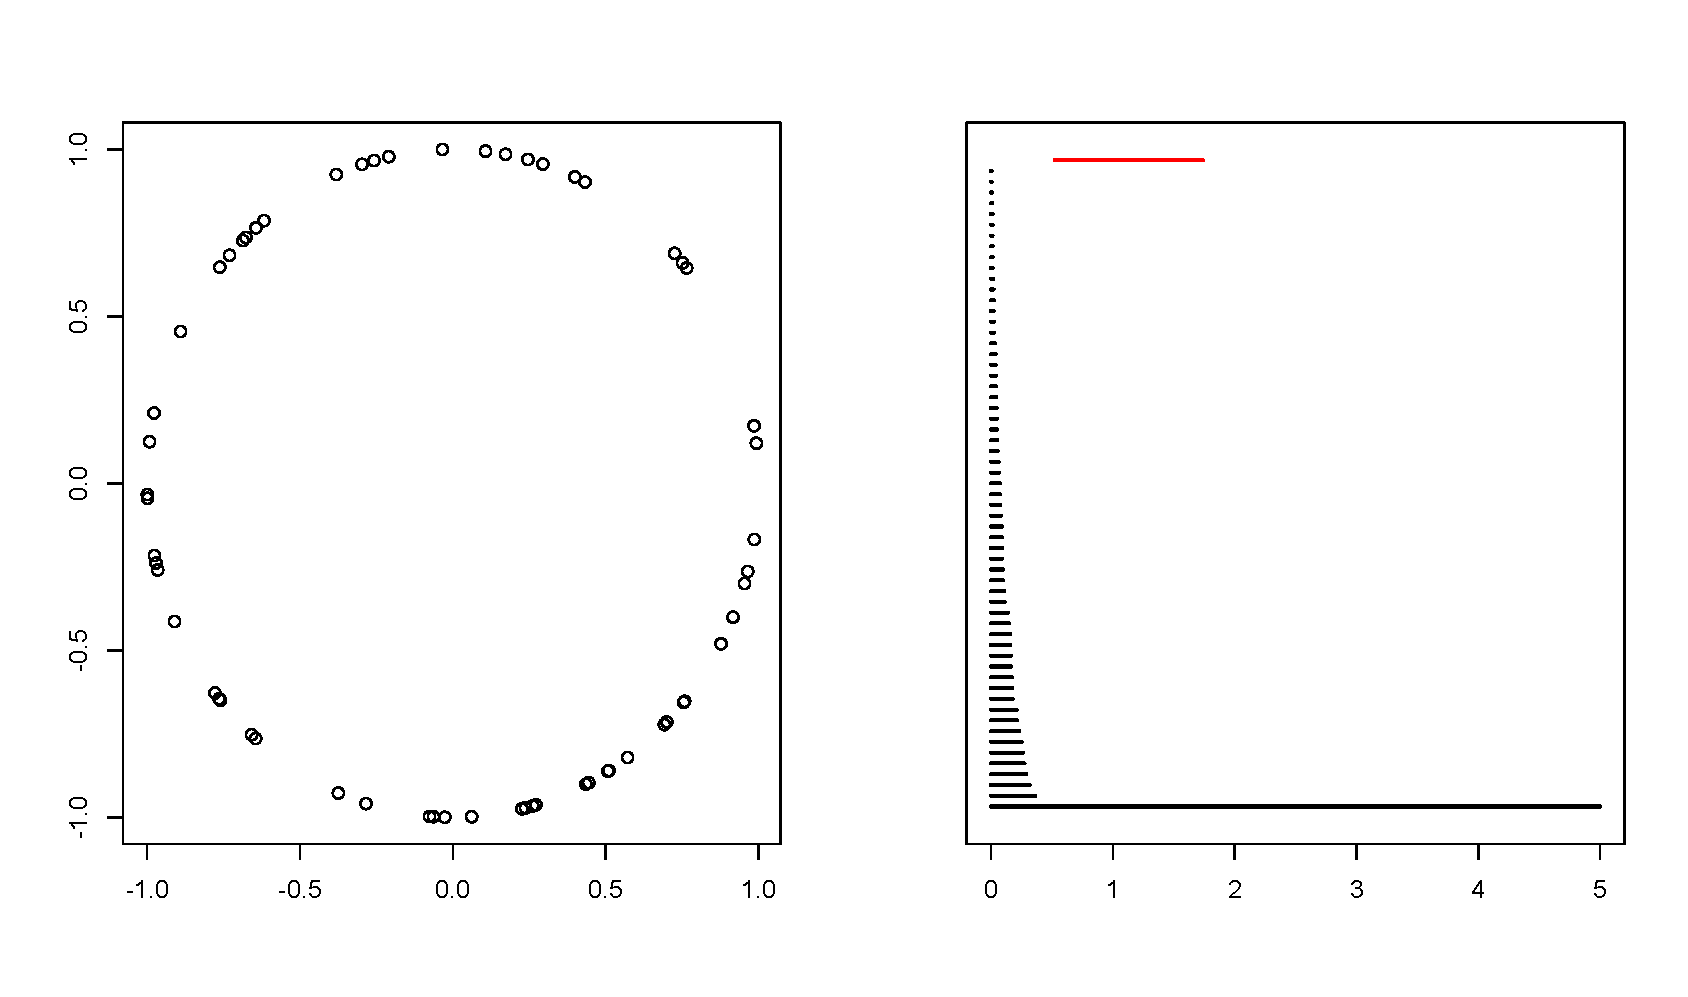
\includegraphics[width=.8\linewidth]{gfx/circle_persistence.pdf}
  \subcaption{Estrazione casuale da un singolo cerchio}
  \centering
  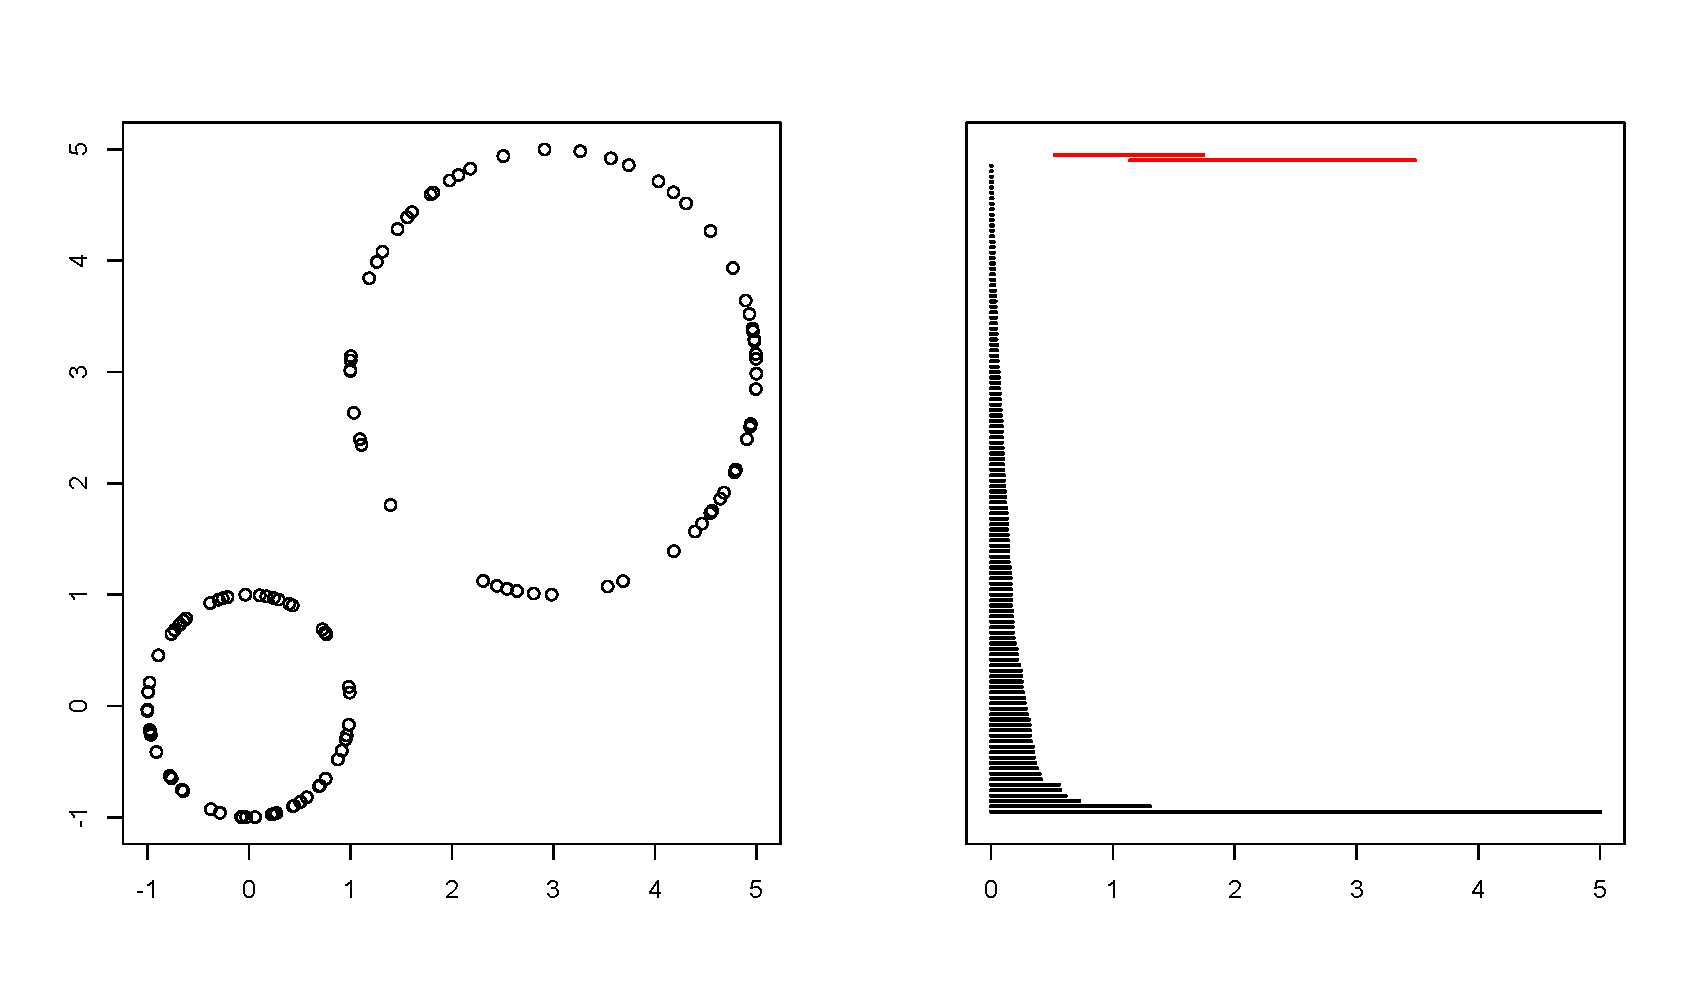
\includegraphics[width=.8\linewidth]{gfx/two_circles.pdf}
  \subcaption{Estrazione casuale da due cerchi}
\end{figure}

Anche in questi casi banali è possibile osservare come la diversa distribuzione dei punti sui cerchi causa interssanti artefatti, come si può osservare dall'omologia persistente 0-dimensionale nel caso dei due cerchi, in cui la presenza di due componenti connesse non è così marcatamente evidente dal codice a barre persistente.

(NMDC: aggiungere toro e sfera)
